\documentclass{report}
\usepackage[utf8]{inputenc}
\usepackage[T1]{fontenc}
\usepackage{graphicx}
\usepackage[francais]{babel} 
\usepackage{array} 

\title{Etat de l'art}
\author{Projet DUT INFO}
\date{17 Septembre 2013}
\begin{document}
\maketitle
\tableofcontents

\part{Introduction}



\chapter{Principe d'affichage d'une image sur ordinateur}
\part{Outils utilisés}

\chapter{OpenGL}

\section{Introduction}
Comme vu précédemment l'affichage de contenu à l'écran par ordinateur consiste en un processus de communication entre le processeur , la carte graphique et l'écran.Ces messages, très bas niveau, sont difficilement utilisables directement par les développeurs.

OpenGL est une Interface de Programmation (API) qui définit un moyen de communication entre l'application et la carte graphique.
Cependant il n'existe aucune implémentation "officielle" d'OpenGL, c'est le rôle de chaque constructeur de l'implémenter sur son matériel.  
Elle contient un ensemble de 150 fonctions qui permettent de définir les objets et opérations nécessaires pour rendre un contexte tri-dimensionnel.
L’avantage d'OpenGL est qu’elle est totalement portable avec tous les systèmes d'exploitation. Ceci est dû au fait qu'elle sert plutôt d'intermédiaire entre l'application et le système d'exploitation. OpenGL sert à faire le rendu et le communiquer à la carte graphique mais ne gère ni le fenêtrage, ni les événements. 
La majorité des bibliothèques graphiques utilisées pour créer des fenetres graphiques gèrent OpenGL, il est donc possible d'utiliser OpenGL dans un contexte SDL, SFML, QT, API Windows.

%Device context ? Rendering context ?

OpenGL est basé sur un principe de primitives : chaque objet est composé de primitives (sommets, faces, polygones) Pour créer un objet, il suffit donc de définir toutes ses primitives

\newcolumntype{M}[1]{>{\raggedright}m{#1}}

\begin{center}
   \begin{tabular}{| c | M{8cm} |}
   	 \hline
     \verb|GL_POINTS| 			& Dessine un point à chaque n vertex  \tabularnewline
     \hline
     \verb|GL_LINE| 			& Dessine une ligne d’un point n à n+1 \tabularnewline
     \hline
     \verb|GL_LINE_STRIP| 		& Dessine un ensemble de lignes connectées d’un vertex à un autre \tabularnewline
     \hline
     \verb|GL_LINE_LOOP| 		& Même chose que \verb|GL_LINE_STRIP|, mais du dernier vertex, on revient au premier. \tabularnewline
     \hline
     \verb|GL_TRIANGLES| 		& Dessine des triangles avec 3 vertex \tabularnewline
     \hline
     \verb|GL_TRIANGLE_STRIP| 	& Dessine une série de triangles avec les n vertexs définis   \tabularnewline
     \verb|GL_TRIANGLE_FAN| 	& Même chose que \verb|GL_TRIANGLE_STRIP|, sauf que le sommet de chaque triangle est le premier vertex défini \tabularnewline
     \hline
     \verb|GL_QUADS| 			& Dessine un quadrilatère avec 4 vertex \tabularnewline
     \hline
     \verb|GL_QUAD_STRIP| 		& Dessine une série de quadrilatères avec les n vertex définis \tabularnewline
     \hline
     \verb|GL_POLYGON| 			& Dessine un polygône générique dont le nombre de segments \verb|n’est| pas prédéterminé \tabularnewline
     \hline
   \end{tabular}
 \end{center}
 
 \begin{center}
	 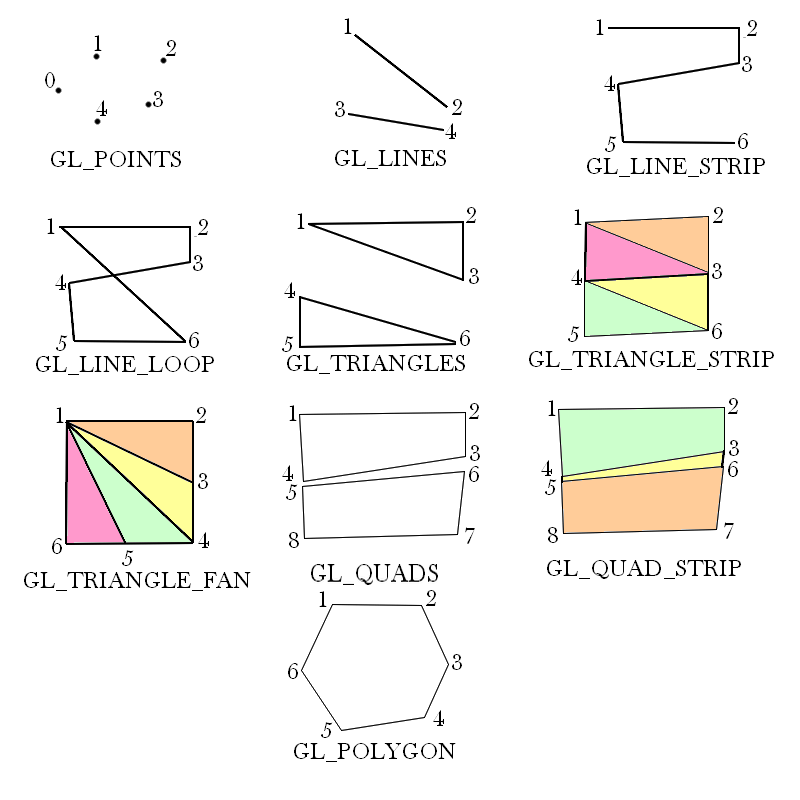
\includegraphics[height=11cm]{img/Primitives}
 \end{center}
\newpage

\section{Fonctionnement d'OpenGL}
\begin{center}
	 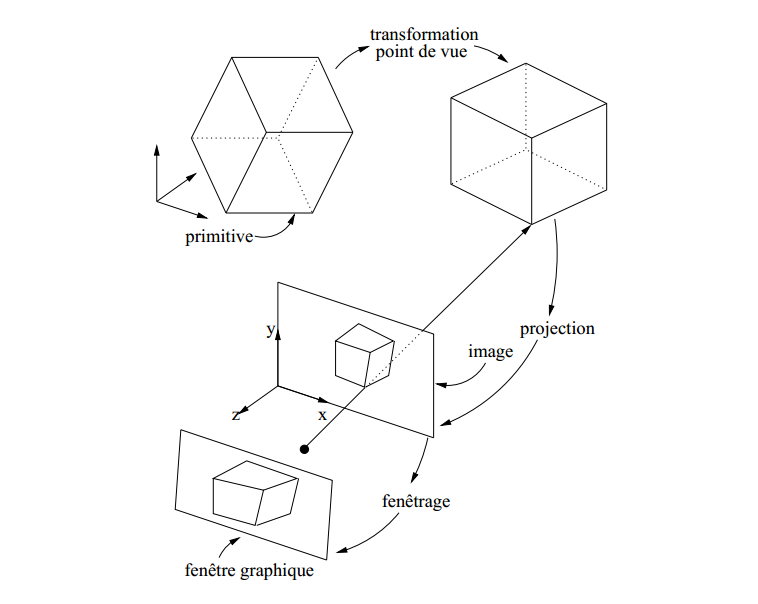
\includegraphics[height=11cm]{img/Fonctionnement}
 \end{center}

La première étape est de définir les primitives des objets à dessiner (x,y,z pour chaque Vertex).
OpenGL dessine une image tampon qui sera soit conservée dans la mémoire vidéo de la fenêtre graphique avant d’être affichée, soit une image tampon intermédiaire, on parle alors de double buffering.

La transformation du point de vue sert à la position du plan image. Elle prend en compte la position de la camera pour se placer correctement autour de l'objet. Ces modifications sont faites à l'aide de matrices. 

Les primitives sont ensuite projetées sur ce plan en fonction des paramètres que l’on a affecté à la projection. Cette projection peut être spécifiée de deux manières. (Voir Projection)

Au final l’image que l’on obtient est redimensionnée en fonction de la taille de la fenêtre graphique . On parle maintenant de pixels et plus de vertex.
\newpage

\subsection{Primitives}
Tout d'abord, il s'agit de définir chaque objet à modeliser, gràce aux primitives précédemment décrites.

Dans le code, chaque primitives est décrite de la manière suivante:


%//////////////////////////////////
%NE PAS TOUCHER A CE TRUC IMMONDE :)
\begin{tabbing}
XXXX\=XXXX\= \kill

\> \verb|glBegin("type_de_primitive");| \\
\> \> glVertex(x,y,x);\\
\> \> . \\
\> \> . On définit chaque vertex en fonction du type de primitive\\
\> \> . \\
\> \> glVertex(x,y,x);\\
\> glEnd();
\end{tabbing}
%NE PAS TOUCHER A CE TRUC IMMONDE :)
%//////////////////////////////////

\subsection{Transformation de point de vue}
La transformation de point de vue consiste en la modification d'une matrice appelée MODELVIEW. Il faut d'abord signaler à OpenGL que l'on veut modifier cette matrice avec la fonction suivante :

\begin{tabbing}
XXXX\= \kill
\> \verb|glMatrixMode( GL_MODELVIEW );|
\end{tabbing}

Ensuite, on charge la matrice identité, ce qui permet de reinitialiser la matrice en cours, puis définit la caméra.

\begin{tabbing}
XXXX\= \kill
\> \verb|glLoadIdentity( );| \\
\> \verb|gluLookAt(eyeX,eyeY,eyeZ,centerX,centerY,centerZ,upX,upY,upZ);|
\end{tabbing}

La définition de la caméra necessite 9 paramètres: les 3 premiers pour placer la caméra dans l'espace (x,y,z), les 3 suivants pour définir le point regardé par la caméra (x,y,z) et les trois derniers pour définir quel est l'axe vertical, en général y (On place seulement l'axe voulu à 1 et les autres à 0).\\\\

Il est possible d'effectuer d'autres opérations sur cette matrice, comme une rotation autour d'un des 3 axes ou une translation de vecteur gràce aux deux fonctions suivantes :

\begin{tabbing}
XXXX\= \kill
\> \verb|glRotatef(angle,x,y,z);| \\\\
Avec l'angle souhaité et x, y et z à 0 ou 1 suivant autour de quel axe on souhaite\\ effectuer la rotation.\\\\
\> \verb|glTranslatef(vX,vY,vZ);|\\\\
Avec vX, vY et vZ les composantes de la translation. 
\end{tabbing}

\subsection{Projection}
\subsection{Image Finale}

%A compléter

\newpage

\chapter{Bibliothèque de rendu 3D}

%A compléter
\part{Problèmes Rencontrés}

\chapter{Optimisation}
\newpage
\end{document}